\documentclass[11pt]{aghdpl}
% \documentclass[en,11pt]{aghdpl}  % praca w języku angielskim

% Lista wszystkich języków stanowiących języki pozycji bibliograficznych użytych w pracy.
% (Zgodnie z zasadami tworzenia bibliografii każda pozycja powinna zostać utworzona zgodnie z zasadami języka, w którym dana publikacja została napisana.)
\usepackage[english,polish]{babel}

% Użyj polskiego łamania wyrazów (zamiast domyślnego angielskiego).
\usepackage{polski}

\usepackage[utf8]{inputenc}

% dodatkowe pakiety

\usepackage{mathtools}
\usepackage{amsfonts}
\usepackage{amsmath}
\usepackage{amsthm}

% --- < bibliografia > ---

\usepackage[
backend=bibtex,
style=numeric,
sorting=none,
%
% Zastosuj styl wpisu bibliograficznego właściwy językowi publikacji.
language=autobib,
autolang=other,
% Zapisuj datę dostępu do strony WWW w formacie RRRR-MM-DD.
urldate=iso8601,
% Nie dodawaj numerów stron, na których występuje cytowanie.
backref=false,
% Podawaj ISBN.
isbn=true,
% Nie podawaj URL-i, o ile nie jest to konieczne.
url=false,
%
% Ustawienia związane z polskimi normami dla bibliografii.
maxbibnames=3,
]{biblatex}

\usepackage{csquotes}
% Ponieważ `csquotes` nie posiada polskiego stylu, można skorzystać z mocno zbliżonego stylu chorwackiego.
\DeclareQuoteAlias{croatian}{polish}

\addbibresource{praca.bib}

% Nie wyświetlaj wybranych pól.
%\AtEveryBibitem{\clearfield{note}}


% ------------------------
% --- < listingi > ---

% Użyj czcionki kroju Courier.
\usepackage{courier}

\usepackage{listings}
\lstloadlanguages{TeX}

\lstset{
	literate={ą}{{\k{a}}}1
           {ć}{{\'c}}1
           {ę}{{\k{e}}}1
           {ó}{{\'o}}1
           {ń}{{\'n}}1
           {ł}{{\l{}}}1
           {ś}{{\'s}}1
           {ź}{{\'z}}1
           {ż}{{\.z}}1
           {Ą}{{\k{A}}}1
           {Ć}{{\'C}}1
           {Ę}{{\k{E}}}1
           {Ó}{{\'O}}1
           {Ń}{{\'N}}1
           {Ł}{{\L{}}}1
           {Ś}{{\'S}}1
           {Ź}{{\'Z}}1
           {Ż}{{\.Z}}1,
	basicstyle=\footnotesize\ttfamily,
}

% ------------------------

\AtBeginDocument{
	\renewcommand{\tablename}{Tabela}
	\renewcommand{\figurename}{Rys.}
}

% ------------------------
% --- < tabele > ---

\usepackage{mdwlist}
\usepackage{array}
\usepackage{tabularx}
\usepackage{multirow}
\usepackage{booktabs}
\usepackage{makecell}
\usepackage{graphicx}
\usepackage[flushleft]{threeparttable}
\usepackage{enumitem}
%\usepackage[section]{placeins}
\usepackage{float}
\usepackage[dvipsnames]{xcolor}

% defines the X column to use m (\parbox[c]) instead of p (`parbox[t]`)
\newcolumntype{C}[1]{>{\hsize=#1\hsize\centering\arraybackslash}X}
\DeclareGraphicsExtensions{.pdf,.png,.jpg}

%---------------------------------------------------------------------------

\author{Bartłomiej Konieczny}
\shortauthor{B. Konieczny}

%\titlePL{Przygotowanie bardzo długiej i pasjonującej pracy dyplomowej w~systemie~\LaTeX}
%\titleEN{Preparation of a very long and fascinating bachelor or master thesis in \LaTeX}

\titlePL{Sztuczna inteligencja na przykładzie symulacji komputerowej}
\titleEN{Artificial intelligence in computer simulation}


\shorttitlePL{Sztuczna inteligencja na przykładzie symulacji komputerowej} % skrócona wersja tytułu jeśli jest bardzo długi
\shorttitleEN{Artificial intelligence in computer simulation}

\thesistype{Praca dyplomowa inżynierska}
%\thesistype{Master of Science Thesis}

\supervisor{dr inż. Mirosław Gajer}
%\supervisor{Marcin Szpyrka PhD, DSc}

\degreeprogramme{Informatyka}
%\degreeprogramme{Computer Science}

\date{2015}

\department{Katedra Informatyki Stosowanej}
%\department{Department of Applied Computer Science}

\faculty{Wydział Elektrotechniki, Automatyki,\protect\\[-1mm] Informatyki i Inżynierii Biomedycznej}
%\faculty{Faculty of Electrical Engineering, Automatics, Computer Science and Biomedical Engineering}

\acknowledgements{}


\setlength{\cftsecnumwidth}{10mm}



\lstnewenvironment{code}[1][]%
  {\noindent\minipage{\linewidth}\medskip 
   \lstset{basicstyle=\ttfamily\footnotesize,frame=single,#1}}
  {\endminipage}


%---------------------------------------------------------------------------
\setcounter{secnumdepth}{4}

\begin{document}

\titlepages

% Ponowne zdefiniowanie stylu `plain`, aby usunąć numer strony z pierwszej strony spisu treści i poszczególnych rozdziałów.
\fancypagestyle{plain}
{
	% Usuń nagłówek i stopkę
	\fancyhf{}
	% Usuń linie.
	\renewcommand{\headrulewidth}{0pt}
	\renewcommand{\footrulewidth}{0pt}
}

\setcounter{tocdepth}{2}
\tableofcontents
\clearpage

\chapter{Wstęp}
\label{cha:wstep}

W ostatniej dekadzie można zauważyć zwiększone zainteresowanie rozwiązaniami z dziedziny
sztucznej inteligencji. Innowacyjne pomysły z użyciem tych algorytmów pozwalają nie tylko na interpretacje ogromnych 
ilości danych, których człowiek nie jest w stanie przetworzyć ale również, między innymi na rozwój 
autonomicznych pojazdów, jeżdżących bez nadzoru kierowcy.\\
Według \cite{mccarthy2007artificial} sztuczną inteligencją możemy nazwać ``badanie i rozwój inteligentnych maszyn, 
w szczególności programów komputerowych''.\\
Inteligentne zachowanie agenta możemy zdefiniować, gdy agent\cite{L.:2010:AIF:1809744}
\begin{itemize*}
 \item dostosowuje swoje zachowanie do aktualnych warunków i celów,
 \item ma zdolność zmiany otoczenia i celów,
 \item uczy się z doświadczenia,
 \item wykonuje odpowiednie do swoich ograniczeń akcję.
\end{itemize*}
Wykorzystując powyższe definicję, sztuczną inteligencje określamy jako dziedzinę naukową zajmującą się badaniem, 
rozwojem i implementacją programów i maszyn wykazujących cechy inteligencji, tzn. takie które ucząc się z 
doświadczenia, będąc zmiennym w stosunku do otaczającego ich otoczenia i warunków dążą do wykonania swoich celów 
uwzględniając obowiązujące je ograniczenia. 
%---------------------------------------------------------------------------

\section{Cele pracy}
\label{sec:celePracy}

Celem pracy jest opis i implementacja inteligentnego agenta. Agent wykorzystując algorytmy uczenia ze wzmacnianiem 
wyciąga wnioski z podejmowanych akcji i dostosowuje swoje zachowanie. W pracy zostanie wyjaśnione również inne rodzaje 
algorytmów uczenia ze wzmocnieniem.


%---------------------------------------------------------------------------

\section{Zawartość pracy}
\label{sec:zawartoscPracy}

Symulacja graficzna przedstawiająca agenta w środowisku.
















\chapter{Uczenie maszynowe - rozdział teoretyczny}
\label{cha:ogolnyrozdzialteoretyczny}

Jednym z najistotniejszych zagadnień z dziedziny sztucznej inteligencji jest uczenie maszynowe. 
Uczenie maszynowe jest metodą analizy danych, która automatyzuje budowę modelu analitycznego na podstawie nauki z 
danych. W wielu zastosowaniach użycie metod uczenia maszynowego jest znacznie bardziej efektywne od manualnego 
programowania, w wyniku czego 
uczenie maszynowe znalazło szerokie zastosowanie w informatyce i innych dziedzinach.
W ostatniej dekadzie można zauważyć zwiększone użycie metod uczenia maszynowego\cite{domingos2012few}.

\section{Podejścia do uczenia maszynowego}
\label{sec:podejsciadouczeniamaszynowego}

\begin{itemize}
 \item uczenie nadzorowane,
 \item uczenie nienadzorowane,
 \item uczenie ze wzmocnieniem,
\end{itemize}

\subsection{Uczenie nadzorowane}
\label{subsec:uczenienadzorowane}

Uczenie nadzorowane polega na wnioskowaniu funkcji z określonych danych trenujących.
Wykorzystując dostarczone przykłady algorytmy potrafią estymować wartości danych, które mogą nie występować w 
podanym zbiorze wejściowym. Dzięki generalizowaniu z przykładów, metody uczenia nadzorowanego są w stanie 
wyznaczać przewidywane wartości na podstawie danych trenujących.

Ważną cechą danych trenujących w uczeniu nadzorowanym jest konieczność ich oznaczenia. Algorytm, aby móc 
szacować pożądane wartości funkcji, musi posiadać wiedzę o ich cechach.

Przykładem zastosowania algorytmów uczenia nadzorowanego jest system rozpoznawania niechcianych wiadomości w klientach 
pocztowych. Danymi wejściowymi są w tym przypadku kategoryzowane na pożądane lub niepożądane wiadomości e-mail.
System generalizując podane mu przykłady jest w stanie zidentyfikować kolejne wiadomości i wykonać odpowiednią akcję, 
zależnie od preferencji użytkownika (może to być na przykład usunięcie lub przeniesienie do zdefiniowanego folderu).

Wiele różnych algorytmów uczenia nadzorowanego zostało wykorzystanych by rozwiązać problem klasyfikacji wiadomości 
e-mail. Użyto między innymi algorytmów k-nearest neighbor\cite{firte2010spam}, Naive 
Bayes\cite{marsono2008binary}\cite{lakshmi2010spam} czy Random Forest\cite{koprinska2007learning}, jednak wiąże 
się to z istotnymi wadami\cite{li2014towards}:

\begin{itemize}
 \item \textbf{Wymagane oznaczenie danych testowych}. Metody uczenia nadzorowanego wymagają, aby dane trenujące były 
oznaczone. W przypadku klasyfikacji wiadomości e-mail, koniecznie jest ich oznaczenie w zależności od tego czy są 
szkodliwe czy nie. Problem stwarza tutaj wielkość danych. Ilość wiadomości, która jest wymieniana w sieci jest 
bardzo duża. W związku z czym, żeby klasyfikacja miała sens, wymagane też jest oznaczenie sporej ilości przykładów, co 
nie zawsze jest możliwe i opłacalne do zrealizowania. 
\item \textbf{Mała liczba danych testowych}. W związku z niewielką (w stosunku do wszystkich możliwych) ilością danych 
trenujących, algorytm jest mało odporny na modyfikowane dane. Osoby rozsyłające niechciane wiadomości bardzo często 
będą zmieniać ich treść i strukturę, na taką, która nigdy nie pojawiła się wśród danych trenujących. Może mieć to 
negatywny wpływ na wynik działania algorytmu.
\end{itemize}


 

\subsection{Uczenie nienadzorowane}
\label{subsec:uczenienienadzorowane}

Podobnie jak w uczeniu nadzorowanym, algorytmy uczenia nienadzorowanego wyznaczają funkcje na podstawie danych 
wejściowych, jednak są w stanie odkryć niewidoczne zależności między nimi. Konsekwencją wynikającą z charakterystyki 
algorytmów uczenia nadzorowanego jest niemożność określenia błędu lub poprawności rozwiązania. Celem działania 
algorytmu może być na przykład kategoryzowanie informacji (klasteryzacja).

W odróżnieniu od uczenia nadzorowanego, metody uczenia nienadzorowanego są w stanie wykryć ukryty wzorzec w danych 
wejściowych.

Używając jako wejścia informacji dotyczących kwiatów irysów w postaci przedstawionej na listingu \ref{lst:danekwiatow}, 
algorytmy uczenia 
nienadzorowanego mogą być zastosowane w celu wywnioskowania gatunku kwiatu (\textit{setosa}, 
\textit{versicolor},  \textit{virginica}) na 
podstawie długości i szerokości płatka  (\textit{sepal}) i listka kielichu (\textit{petal}).

\begin{code}[caption=Przykład danych o kwiatach irysów, label={lst:danekwiatow}, captionpos=b, 
belowcaptionskip=4pt]
    Sepal.Length Sepal.Width Petal.Length Petal.Width    Species
1            5.1         3.5          1.4         0.2     setosa
2            4.9         3.0          1.4         0.2     setosa
3            4.7         3.2          1.3         0.2     setosa
4            4.6         3.1          1.5         0.2     setosa
53           6.9         3.1          4.9         1.5 versicolor
54           5.5         2.3          4.0         1.3 versicolor
55           6.5         2.8          4.6         1.5 versicolor
56           5.7         2.8          4.5         1.3 versicolor
101          6.3         3.3          6.0         2.5  virginica
102          5.8         2.7          5.1         1.9  virginica
103          7.1         3.0          5.9         2.1  virginica
104          6.3         2.9          5.6         1.8  virginica
\end{code}
\\\\\\
Na rys. \ref{fig:plotsepalwidthsepallength}, przedstawione zostało rozmieszczenie gatunków kwiatów w zależności od 
długości i szerokości płatka kwiatu. Wyraźnie widać podział na dwa podstawowe klastry
\begin{itemize*} 
\renewcommand{\labelitemi}{$\bullet$}
 \item gatunek setosa,
 \item gatunek versicolor i virginica.
\end{itemize*}

\begin{figure}[h]
    \centering
    \textbf{Rozmieszczenie kwiatów irysów}\par\medskip
    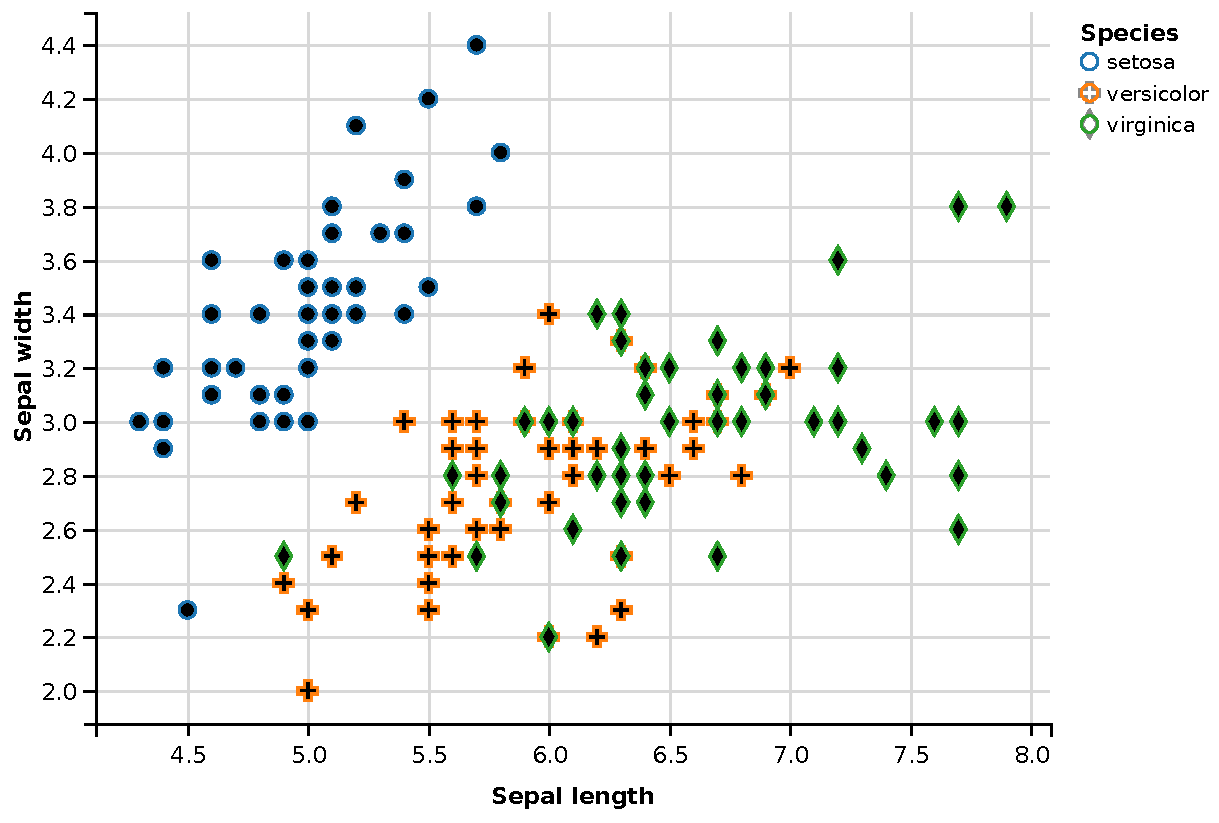
\includegraphics[scale=0.5]{plotsepalwidthsepallength}
    \caption{Populacja kwiatów irysów w zależności od szerokości i długości płatka kwiatu}
    \label{fig:plotsepalwidthsepallength}
\end{figure}

Stosując algorytmy uczenia nienadzorowanego, nie wiemy w jaki sposób klasyfikować dane trenujące. W tym celu możemy 
wykorzystać algorytm k-means\cite{coates2012learning}, który na podstawie określonych cech grupuje dane w podaną liczbę 
klastrów.
Poddając przedstawione dane działaniu algorytmu k-means, uzyskujemy wynik przedstawiony na rys. \ref{fig:cluster2} oraz 
rys. \ref{fig:cluster3}.


\begin{figure}[h!]
    \centering
    \textbf{Wynik działania algorytmu k-means}\par\medskip
    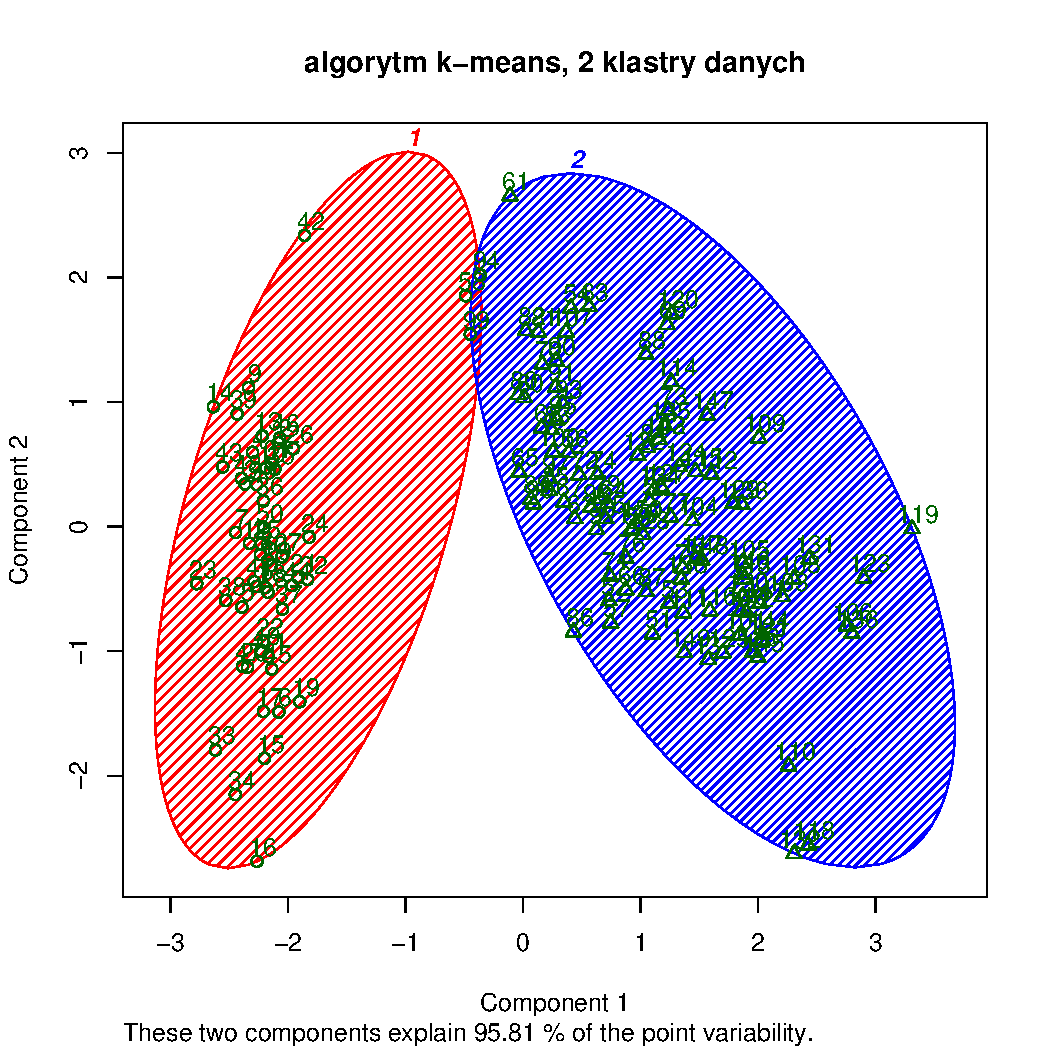
\includegraphics[scale=0.5]{cluster2}
    \caption{Wynik działania algorytmu klasteryzacji k-means dla 2 klastrów kwiatów irysów w zależności od szerokości i 
długości płatka kwiatu}
    \label{fig:cluster2}
\end{figure}

\begin{figure}[h!]
    \centering
    \textbf{Wynik działania algorytmu k-means}\par\medskip
    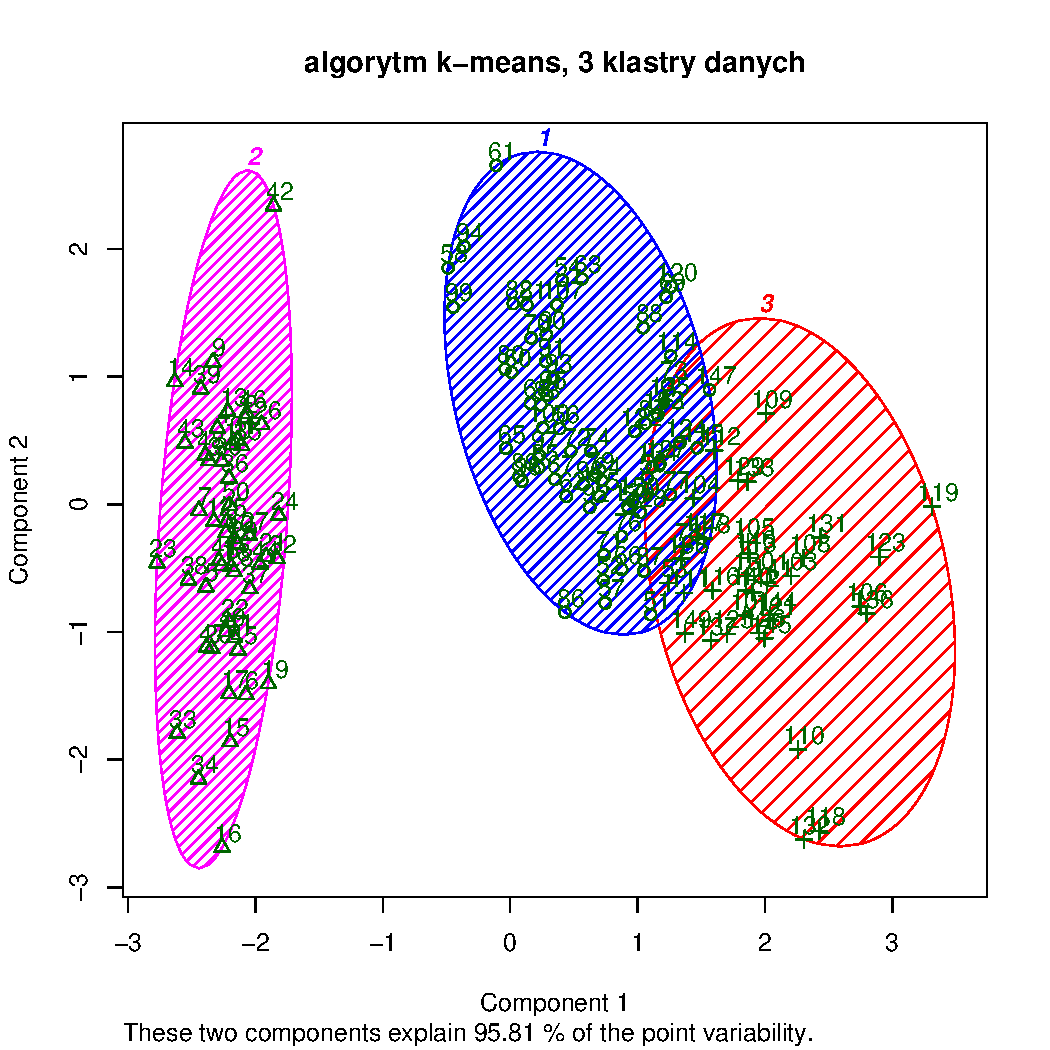
\includegraphics[scale=0.4]{cluster3}
    \caption{Wynik działania algorytmu klasteryzacji k-means dla 3 klastrów kwiatów irysów w zależności od szerokości i 
długości płatka kwiatu}
    \label{fig:cluster3}
\end{figure}


Na rys. \ref{fig:cluster2} można zaobserwować, że algorytm zadziała z dużą skutecznością rozróżniając pomiędzy dwoma 
gatunkami dla dwóch klastrów, tj. pomiędzy gatunkiem setosa, a gatunkami versicolor i virginica, jednak algorytm będzie 
miał problem rozróżnić pomiędzy gatunkami versicolor i virginica.
W tym celu można zbiór podzielić na trzy klastry jak na rys.\ref{fig:cluster3}, ale nie gwarantuje to 
wystarczającej skuteczności przydziału. \\
Tym samym można zaobserwować, że gatunek versicolor i virginica nie są 
rozróżnialne, używając przedstawionych danych wejściowych.\\
Rozważając sytuacje, w której dodana by została duża liczba dodatkowych wpisów, różnych od aktualnych danych, 
można by było zaobserwować pojawienie się kolejnego klastra danych, co oznacza pojawienie się nowego gatunku kwiatu.


\subsection{Uczenie ze wzmocnieniem}
\label{subsec:uczeniezewzmocnieniem}

Uczenie ze wzmocnieniem jest obszarem uczenia maszynowego, w którym inteligentny agent wykonując akcję w otoczeniu otrzymuje odpowiednią nagrodę.
Robot decyduje jaka akcja zostanie wykonana na podstawie istniejącej polityki. Algorytmy uczenia ze wzmocnieniem nie 
wymagają danych trenujących by wykonać swoje zadanie. Na podstawie wiedzy o stanie otoczenia, możliwych do wykonania 
akcji w danym stanie oraz funkcji nagrody, która agent otrzymuje za wykonanie danych akcji, robot, ucząc się metodą 
prób i błędów odkrywa sposoby wybierania kolejnych akcji (polityki) tak, aby osiągnąć swój cel.

\begin{figure}[h]
    \centering
    \textbf{Uczenie ze wzmocnieniem}\par\medskip
    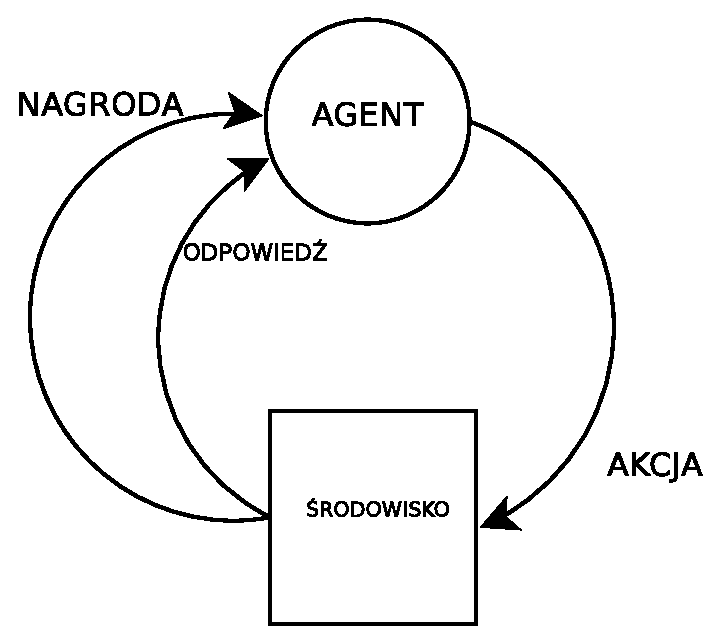
\includegraphics[scale=0.8]{DIAGRAMreinforcementlearning}
    \caption{Schemat uczenia ze wzmocnieniem}
    \label{fig:DIAGRAMreinforcementlearning}
\end{figure}

Na rys. \ref{fig:DIAGRAMreinforcementlearning} przedstawiono schemat współpracy agenta ze środowiskiem. Agent 
podejmując akcję w otoczeniu dostaje nagrodę za podjętą decyzję w danym stanie, oraz informacje o nowym, aktualnym 
stanie środowiska (otoczenie może ulec zmianie po wykonaniu przez robota akcji).

Algorytmy uczenia ze wzmocnieniem dotyczą specyficznych zadań występujących w uczeniu maszynowym. Problem polega na 
odnalezieniu przez agenta optymalnej akcji do wykonania na podstawie wiedzy o aktualnym jego stanie. W przypadku, 
gdy to działanie jest powtórzone, możemy mówić o MDP (Procesy decyzyjne Markowa).

Procesem decyzyjnym Markowa nazywamy model środowiska w algorytmach uczenia ze wzmocnieniem, oznaczamy go jako:\\
$$MDP = (S, A, P(s, s'), R(r, r'), \gamma)$$
gdzie
\begin{enumerate}
 \item $S$ to zbiór stanów
 \item $A$ zbiór możliwych akcji
 \item $P(s, s')$ prawdopodobieństwo przejścia do stanu $s'$ ze stanu $s$ po wykonaniu akcji $a$, w czasie $t$
 \item $R(r, r')$ nagroda po przejściu do stanu $s'$ ze stanu $s$
 \item $\gamma$ współczynnik regulujący stosunek między nagrodami przewidywanymi w późniejszym czasie i 
otrzymywanymi aktualnie, $0 < \gamma < 1$
\end{enumerate}

Zadaniem MDP jest uzyskanie takiej polityki robota, która zmaksymalizuje sumę otrzymywanych nagród.

$$\sum\limits_{t=0}^\infty \gamma^{t} R_{a_{t}}(s_{t}, s_{t+1})$$

Algorytmy uczenia ze wzmocnieniem znalazły zastosowanie między innymi w implementacji autonomicznego 
helikoptera\cite{abbeel2007application}, udoskonaleniu działania windy\cite{barto1996improving}, usprawnienia 
sygnalizacji świetlnej\cite{wiering2000multi} czy budowie inteligentnego robota\cite{kimura2001reinforcement}.


\section{Podsumowanie}

Uczenie nienadzorowane posiada tę przewagę nad uczniem nadzorowanym, że nie wymaga oznaczenia danych trenujących 
oraz potrafi wykryć ukryte zależności pomiędzy cechami przykładów. Jednak w odróżnieniu od obydwu metod, uczenie ze 
wzmacnianiem jest odmienne w tym, że nie wymaga podawania jakichkolwiek danych przykładowych, a jedynie na podstawie 
zdefiniowanych nagród i akcji, agent uczy się odpowiedniego działania.
By zaimplementować robota uczącego się wykonywania akcji w otoczeniu wybrano implementacje metod uczenia ze 
wzmacnianiem, ze względu na charakterystykę środowiska odpowiadającą wymaganiom procesów decyzyjnych Markowa.













\chapter{Implementacja}
\label{cha:implementacja}

Implementacja

\section{Opis implementacji}
\label{sec:opisimplementacji}

\subsection{Wybór algorytmów}
\label{subsec:wyboralgorytmow}

\subsubsection{Q-learning}
\label{subsubsec:qlearning}

\subsubsection{SARSA}
\label{subsubsec:sarsa}

\section{Wykorzystane technologie}
\label{sec:wykorzystanetechnologie}

Java 8 (środowisko IntelliJ Idea)
LibGdx (symulacja graficzna)
Project Lombok
Apache POI(czytanie i zapisywanie do xml)

\section{Symulacja graficzna}
\label{sec:symulacjagraficzna}

Proste prezentacja robota, środowiska
(przeszkoda, nagroda) w postaci figur
geometrycznych
Zamknięta przestrzeń dwuwymiarowa, po
której może się poruszać agent.

Akcje: MOVE_UP, MOVE_DOWN,
MOVE_RIGHT, MOVE_LEFT
● Reprezentacja stanu
siatka 3x3

\section{Napotkane problemy}
\label{sec:napotkaneproblemy}

Reprezentacja stanu
Testowanie działania algorytmów

\section{Wynik działania}
\label{sec:wynikdzialania}


%---------------------------------------------------------------------------















\chapter{Podsumowanie}
\label{cha:podsumowanie}

Zaimplementowany agent poprawnie nauczył się osiągać cel w zaprojektowanym środowisku. Odpowiednio zaimplementowany 
algorytm Q-learning pozwolił robotowi na efektywne generowanie wyników tablicy $Q(S, A)$, dzięki czemu bardzo szybko 
odnalazł optymalną drogę do osiągnięcia stanu końcowego. Ze względu na prostotę środowiska agent 
zaledwie po około siódmej iteracji osiąga najkorzystniejszy wynik. Dla lepszych testów działania algorytmu w 
przyszłości odpowiednie byłoby wprowadzenie bardziej zaawansowanej struktury środowiska. Analogicznie istotną kwestią 
byłby poprawny dobór parametrów algorytmu Q-learning oraz usprawniona reprezentacja stanu.
%\chapter{Wprowadzenie}
\label{cha:wprowadzenie}

\LaTeX~jest systemem składu umożliwiającym tworzenie dowolnego typu dokumentów (w~szczególności naukowych i technicznych) o wysokiej jakości typograficznej (\cite{Dil00}, \cite{Lam92}). Wysoka jakość składu jest niezależna od rozmiaru dokumentu -- zaczynając od krótkich listów do bardzo grubych książek. \LaTeX~automatyzuje wiele prac związanych ze składaniem dokumentów np.: referencje, cytowania, generowanie spisów (treśli, rysunków, symboli itp.) itd.

\LaTeX~jest zestawem instrukcji umożliwiających autorom skład i wydruk ich prac na najwyższym poziomie typograficznym. Do formatowania dokumentu \LaTeX~stosuje \TeX a (wymiawamy 'tech' -- greckie litery $\tau$, $\epsilon$, $\chi$). Korzystając z~systemu składu \LaTeX~mamy za zadanie przygotować jedynie tekst źródłowy, cały ciężar składania, formatowania dokumentu przejmuje na siebie system.

%---------------------------------------------------------------------------

\section{Cele pracy}
\label{sec:celePracy}


Celem poniższej pracy jest zapoznanie studentów z systemem \LaTeX~w zakresie umożliwiającym im samodzielne, profesjonalne złożenie pracy dyplomowej w systemie \LaTeX.

\subsection{Jakiś tytuł}

\subsubsection{Jakiś tytuł w subsubsection}


\subsection{Jakiś tytuł 2}

%---------------------------------------------------------------------------

\section{Zawartość pracy}
\label{sec:zawartoscPracy}

W rodziale~\ref{cha:pierwszyDokument} przedstawiono podstawowe informacje dotyczące struktury dokumentów w \LaTeX u. Alvis~\cite{Alvis2011} jest językiem 



















%\chapter{Pierwszy dokument}
\label{cha:pierwszyDokument}

W rozdziale tym przedstawiono podstawowe informacje dotyczące struktury prostych plików \LaTeX a. Omówiono również metody kompilacji plików z zastosowaniem programów \emph{latex} oraz \emph{pdflatex}.

%---------------------------------------------------------------------------

\section{Struktura dokumentu}
\label{sec:strukturaDokumentu}

Plik \LaTeX owy jest plikiem tekstowym, który oprócz tekstu zawiera polecenia formatujące ten tekst (analogicznie do języka HTML). Plik składa się z dwóch części:
\begin{enumerate}%[1)]
\item Preambuły -- określającej klasę dokumentu oraz zawierającej m.in. polecenia dołączającej dodatkowe pakiety;

\item Części głównej -- zawierającej zasadniczą treść dokumentu.
\end{enumerate}


\begin{lstlisting}
\documentclass[a4paper,12pt]{article}      % preambuła
\usepackage[polish]{babel}
\usepackage[utf8]{inputenc}
\usepackage[T1]{fontenc}
\usepackage{times}

\begin{document}                           % część główna

\section{Sztuczne życie}

% treść
% ąśężźćńłóĘŚĄŻŹĆŃÓŁ

\end{document}
\end{lstlisting}

Nie ma żadnych przeciwskazań do tworzenia dokumentów w~\LaTeX u w~języku polskim. Plik źródłowy jest zwykłym plikiem tekstowym i~do jego przygotowania można użyć dowolnego edytora tekstów, a~polskie znaki wprowadzać używając prawego klawisza \texttt{Alt}. Jeżeli po kompilacji dokumentu polskie znaki nie są wyświetlane poprawnie, to na 95\% źle określono sposób kodowania znaków (należy zmienić opcje wykorzystywanych pakietów).


%---------------------------------------------------------------------------

\section{Kompilacja}
\label{sec:kompilacja}


Załóżmy, że przygotowany przez nas dokument zapisany jest w pliku \texttt{test.tex}. Kolejno wykonane poniższe polecenia (pod warunkiem, że w pierwszym przypadku nie wykryto błędów i kompilacja zakończyła się sukcesem) pozwalają uzyskać nasz dokument w formacie pdf:
\begin{lstlisting}
latex test.tex
dvips test.dvi -o test.ps
ps2pdf test.ps
\end{lstlisting}
%
lub za pomocą PDF\LaTeX:
\begin{lstlisting}
pdflatex test.tex
\end{lstlisting}

Przy pierwszej kompilacji po zmiane tekstu, dodaniu nowych etykiet itp., \LaTeX~tworzy sobie spis rozdziałów, obrazków, tabel itp., a dopiero przy następnej kompilacji korzysta z tych informacji.

W pierwszym przypadku rysunki powinny być przygotowane w~formacie eps, a~w~drugim w~formacie pdf. Ponadto, jeżeli używamy polecenia \texttt{pdflatex test.tex} można wstawiać grafikę bitową (np. w formacie jpg).



%---------------------------------------------------------------------------

\section{Narzędzia}
\label{sec:narzedzia}


Do przygotowania pliku źródłowego może zostać wykorzystany dowolny edytor tekstowy. Niektóre edytory, np. Emacs, mają wbudowane moduły ułatwiające składanie tekstów w LaTeXu (kolorowanie składni, skrypty kompilacji, itp.).

Jednym z bardziej znanych środowisk do składania dokumentów  \LaTeX a jest {\em Kile}. Aplikacja dostępna jest dla środowiska KDE począwszy od wersji 2. Zawiera edytor z podświetlaną składnią, zestawy poleceń \LaTeX a, zestawy symboli matematycznych, kreatory tabel, macierzy, skrypty kompilujące i konwertujące podpięte są do poleceń w menu aplikacji (i pasków narzędziowych), dostępne jest sprawdzanie pisowni, edytor obsługuje projekty (tzn. dokumenty składające się z~wielu plików), umożliwia przygotowanie i~zarządzanie bibliografią, itp.

Na stronie \underline{\texttt{http://kile.sourceforge.net/screenshots.php}} zamieszczono kilkanaście zrzutów ekranu środowiska {\em Kile}, które warto przejrzeć, by wstępnie zapoznać się z~możliwościami programu.

Bardzo dobrym środowiskiem jest również edytor gEdit z wtyczką obsługującą \LaTeX a. Jest to standardowy edytor środowiska Gnome. Po instalacji wtyczki obsługującej \LaTeX a, edytor nie ustępuje funkcjonalnościom środowisku Kile, a jest zdecydowanie szybszy w działaniu. Lista dostępnych wtyczek dla tego edytora znajduje się pod adresem \underline{\texttt{http://live.gnome.org/Gedit/Plugins}}. Inne polecane wtyczki to: 
\begin{itemize}
\item Edit shortcuts -- definiowanie własnych klawiszy skrótu;
\item Line Tools -- dodatkowe operacje na liniach tekstu;
\item Multi-edit -- możliwość jednoczesnej edycji w wielu miejscach tekstu;
\item Zoom -- zmiana wielkości czcionki edytora z użyciem rolki myszy;
\item Split View -- możliwość podziału okna edytora na 2 części. 
\end{itemize}



%---------------------------------------------------------------------------

\section{Przygotowanie dokumentu}
\label{sec:przygotowanieDokumentu}

Plik źródłowy \LaTeX a jest zwykłym plikiem tekstowym. Przygotowując plik
źródłowy warto wiedzieć o kilku szczegółach:

\begin{itemize}
\item
Poszczególne słowa oddzielamy spacjami, przy czym ilość spacji nie ma znaczenia.
Po kompilacji wielokrotne spacje i tak będą wyglądały jak pojedyncza spacja.
Aby uzyskać {\em twardą spację}, zamiast znaku spacji należy użyć znaku {\em
tyldy}.

\item
Znakiem końca akapitu jest pusta linia (ilość pusty linii nie ma znaczenia), a
nie znaki przejścia do nowej linii.

\item
\LaTeX~sam formatuje tekst. \textbf{Nie starajmy się go poprawiać}, chyba, że
naprawdę wiemy co robimy.
\end{itemize} 



%\chapter{Przykłady elementów pracy dyplomowej}

\section{Liczba}

Pakiet \texttt{siunitx} zadba o to, by liczba została poprawnie sformatowana: \\
\begin{center}
	\num{1234567890.0987654321}
\end{center}


\section{Rysunek}

Pakiet \texttt{subcaption} pozwala na umieszczanie w podpisie rysunku odnośników do ,,podilustracji'': \\

\begin{figure}[h]
	\centering
	\begin{subfigure}{0.35\textwidth}
		\centering
		\framebox[2.0\width]{A}
		\subcaption{\label{subfigure_a}}
	\end{subfigure}
	\begin{subfigure}{0.35\textwidth}
		\centering
		\framebox[2.0\width]{B}
		\subcaption{\label{subfigure_b}}
	\end{subfigure}
	
	\caption{\label{fig:subcaption_example}Przykład użycia \texttt{\textbackslash subcaption}: \protect\subref{subfigure_a} litera A, \protect\subref{subfigure_b} litera B.}
\end{figure}

\section{Tabela}

Pakiet \texttt{threeparttable} umożliwia dodanie do tabeli adnotacji: \\

\begin{table}[h]
	\centering
	
	\begin{threeparttable}
		\caption{Przykład tabeli}
		\label{tab:table_example}
		
		\begin{tabularx}{0.6\textwidth}{C{1}}
			\toprule
			\thead{Nagłówek\tnote{a}} \\
			\midrule
			Tekst 1 \\
			Tekst 2 \\
			\bottomrule
		\end{tabularx}
		
		\begin{tablenotes}
			\footnotesize
			\item[a] Jakiś komentarz\textellipsis
		\end{tablenotes}
		
	\end{threeparttable}
\end{table}

\section{Wzory matematyczne}

Czasem zachodzi potrzeba wytłumaczenia znaczenia symboli użytych w równaniu. Można to zrobić z użyciem zdefiniowanego na potrzeby niniejszej klasy środowiska \texttt{eqwhere}.

\begin{equation}
E = mc^2
\end{equation}
gdzie
\begin{eqwhere}[2cm]
	\item[$m$] masa
	\item[$c$] prędkość światła w próżni
\end{eqwhere}

Odległość półpauzy od lewego marginesu należy dobrać pod kątem najdłuższego symbolu (bądź listy symboli) poprzez odpowiednie ustawienie parametru tego środowiska (domyślnie: 2 cm).

%\chapter{Testy}

\section{Test URL-a}

Wejdź na stronę \url{https://www.google.pl/} i wpisz szukane zdanie.

\clearpage

\section{Test dzielenia wdów}

Lorem ipsum dolor sit amet, ex est alia dolorem commune. Duo modo errem no. Ea harum doming atomorum mei. Consul animal malorum cu qui, sumo dicta graece an est, vim ei clita regione.

Vel eu quando doming fastidii, mei graeco indoctum an, legere theophrastus in pro. Te mei probatus eleifend interpretaris. Est no autem liber vituperatoribus, cu mea dicam constituto. Ea laudem tritani consectetuer sit, sanctus patrioque expetendis vix in. Duo id fugit adversarium signiferumque, an quot modus molestiae qui.

Ut paulo definiebas pro. Mea an quod esse. Et atomorum facilisis moderatius sit. Graeco iudicabit forensibus in vel. Eam cu lorem aeterno offendit, cu vix nulla congue posidonium. Vel lucilius evertitur vituperata no.

Mea eu graecis prodesset. Et tota eius nec. Ei etiam oratio has, vel ei homero eripuit invenire. Sed ex errem intellegebat, sea et elitr intellegat constituto. Nostro voluptua accusamus eos in, ei sale admodum has. Vim ne consetetur reformidans, ad has malis recusabo persequeris, per etiam virtute invenire in.

Te nihil eruditi eam, sit aperiam accusam mediocritatem at. Nec ne nonumy dictas disputationi, vis ridens sadipscing ex. Harum euripidis ex vix, at consetetur instructior signiferumque mel, at mei elitr honestatis. Id sit congue vituperata. Temporibus eloquentiam no eum.

Pro id esse phaedrum, nostro iudicabit eos ut. Sit ea aperiam alienum, harum audiam voluptua cu usu. Iudico invenire te vel, id suscipit disputando pri. Ut sumo expetenda mea.

Cum at idque nullam aperiam, vis ex aeque ponderum luptatum. Vix soluta graeco dissentiet ut, ut est reque periculis similique, ut dicta dicant repudiare sea. Ne dolor legendos signiferumque ius, at eirmod convenire qui. Suas numquam conceptam mei ex. Autem homero eos et, sea dicta alienum iudicabit ut.

Ea duo consulatu vulputate, id elit perpetua cum. His ei aeque saepe audiam. Prompta laoreet facilisi ne sed, per hinc consetetur te, oratio fuisset ullamcorper mel at. Quis suscipiantur ne nec, agam efficiendi usu in.

Vis eu iuvaret singulis appellantur, usu ex saepe omittantur. Sed possit mnesarchum at, usu illum choro oratio in, et debet dolor vix. Mel aperiri suscipiantur ne, te per illum fuisset, lorem pericula mei ad. Pri id tale lucilius dissentiet, id sea sonet expetenda. Agam sensibus persequeris sed no, eum at tamquam sanctus.

Omnis exerci soleat ut vis. Rebum vidisse sea ex. Ius animal gubergren efficiantur ad, mollis probatus nec ut. Meis platonem ex vel, ut qui tale tritani equidem. Vide meis fuisset mel at, nam an assum delenit gubergren. No illum reprimique vim, te augue nullam per, ludus dicant suscipiantur ne sed.

An pri mediocrem deseruisse, ad sumo audire dissentiet sit. Sit ea civibus lobortis. Etiam ceteros commune ei vis. Pro ei equidem vivendo. Quo ne prima periculis omittantur, ex rebum veritus sit, ei dolor maiestatis mea.

\subsection{Lorem ipsum}

Et mel munere quodsi sapientem. Essent legimus ne pro. Est ornatus definiebas et. No habemus docendi ius, purto sapientem mei at. Tamquam vivendo necessitatibus has at, no habemus praesent nec. No quo modus iudicabit scriptorem. Modus intellegebat ea vim. Cu ius lorem regione offendit, ne accusata sensibus vituperatoribus quo. Sit ut iuvaret indoctum. Ut mea sale justo. Sapientem definitionem ius eu, at sea quem doming. Facete conclusionemque ut nec, vix at duis eius. Eos quot consequuntur et, ornatus liberavisse ne mei.

Per an dicam commodo tractatos, usu in timeam numquam tacimates. Case delectus eu sea, usu audiam eleifend tincidunt id, nec at decore discere mentitum. Ut elit veri eloquentiam his, ceteros tractatos ea has. Duo impetus scribentur et, eu quo errem everti, ad recusabo consulatu ius. Fastidii comprehensam pri ea, ex duo augue quando denique. Eos aeterno deserunt sententiae cu, ius quas tation patrioque ex.

Id autem scripta explicari nec, congue quidam possit te sit. Et usu ipsum bonorum graecis, ferri verear deterruisset eum cu. Purto porro accommodare cu vim. Cum ei tritani pertinacia voluptaria.

\printbibliography

\end{document}
